% !TeX spellcheck = en_US

\chapter{Software Design}
This chapter discusses the possible solutions for working with GIS inside the LIFE simulation system.



\section{Current state}
Currently the GIS support inside MARS is partial, some components of the environment are capable of handling GIS, while others are not currently supporting it.


\subsection{Web browser Front-end}
The WebUI supports GIS for importing and managing this kind of data. It's successor the teaching UI currently does not support GIS. Due to the micro-service structure of the back-end services it is possible for the front-ends to coexist.

\subsection{Back-end Services}
The back-end services fully support GIS. The file service accepts the uploaded files and hands control over to the GIS Data Service (GDS). 

\subsubsection{GIS Data Service}
The GDS is capable of handling the most common GIS types, these are Geotiff and Esri AsciiGrid for raster and Shapefile for vector files. The files may be provided compressed inside a .zip file or as plain files.\\
During the import the GDS determines the type of data automatically by checking the file extension. Once detected, the file is validated and the spatial reference is determined. In case of a valid geo-referenced input, the file is imported into the GeoServer for persistence.


\subsubsection{GeoServer} \label{sec:GS}
The GeoServer (GS) is an open source software that is tailored to store, manage and share GIS. It offers a web GUI as well as a REST API for interaction. The api is structured in a way that it implements common Open Geospatial Consortium (OGC) standards for retrieving data.\\
The Web Feature Service (WFS) allows to retrieve features of vector data, Web Coverage Service (WCS) enables downloading raster data and the Web Map Service (WMS) can generate a tile map for viewing GIS on a map.\\
The GS is build for working with few files and a small number of users. The MARS use-case requires to read thousands to millions of  single values in parallel in a short amount of time. The GS does not satisfy this demands. The retrieval of single values is not supported, since the general use-case is to work with complete files. The performance for retrieving data is also very poor which will require a better solution.


\subsection{GIS Layer}
The GIS Layer inside MARS LIFE reads the Data provided by the GDS and uses it inside the simulation. Since the migration from C\# to .NET Core inside LIFE the GIS layer is not compatible anymore.\\
The current models therefore do not leverage GIS for their input. Data is being transfered into other formats to work around these shortcomings. Vector data is mainly represented as comma separated values (.csv) files and raster data are represented in custom formats.


\section{Solutions}
As mentioned in section \ref{sec:GS} reading data from the GS during the simulation is not feasible inside a high performance environment.\\
Different alternative solutions have been discovered and evaluated. The data could be stored inside a spatial database that is optimized for parallel reads of single values or the GIS file could be supplied to the Simulation and stored in memory for fast reading.

\begin{table}[]
	\centering
	\caption{GIS solutions feature comparison}
	\label{fig:feature_comparison}
	\begin{tabular}{|l|l|l|l|}
	\hline \textbf{Name}	& \textbf{Raster support} & \textbf{Vector support} & \textbf{Type} \\
	\hline GeoServer & yes & yes & self-hosted product \\
	\hline PostGIS	& yes* & yes & Database \\
	\hline MongoDB	& no & yes & Database \\
	\hline Dotspatial & yes & yes & C\# library \\
	\hline NetTopologySuite	& no & yes & C\# library \\
	\hline
	\end{tabular}
\end{table}

\subsection{PostGIS}
Large file: out of memory. Limit to 7 parallel threads solves it, but took 342,197ms

\subsection{MongoDB}


\subsection{Local library}



\section{Performance comparison}

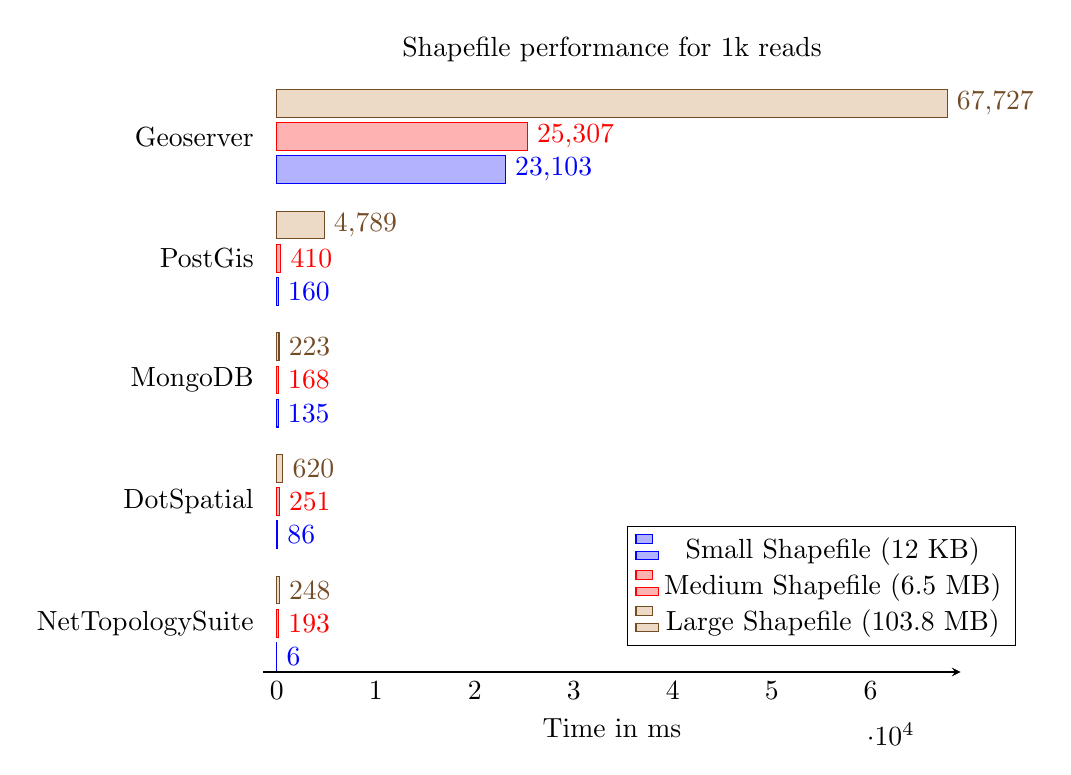
\begin{tikzpicture}
\begin{axis}[
title  = Shapefile performance for 1k reads,
xbar,
y axis line style = { opacity = 0 },
axis x line       = bottom,
tickwidth         = 0pt,
%	enlarge y limits  = 0.02,
enlarge x limits  = 0.02,
symbolic y coords = {NetTopologySuite, DotSpatial, MongoDB, PostGis, Geoserver},
nodes near coords,
height=9cm,
legend style={at={(0.8,0.25)},anchor=north},
xlabel={Time in ms},
]
% Small Shapefile
\addplot coordinates {
	(23103,Geoserver)
	(160,PostGis)
	(135,MongoDB)
	(86,DotSpatial)
	(6,NetTopologySuite)
};
% Mid Shapefile
\addplot coordinates {
	(25307,Geoserver)
	(410,PostGis)
	(168,MongoDB)
	(251,DotSpatial)
	(193,NetTopologySuite)
};
% Large Shapefile
\addplot coordinates {
	(67727,Geoserver)
	(4789,PostGis)
	(223,MongoDB)
	(620,DotSpatial)
	(248,NetTopologySuite)
};
\legend{Small Shapefile (12 KB), Medium Shapefile (6.5 MB), Large Shapefile (103.8 MB)}
\end{axis}
\end{tikzpicture}

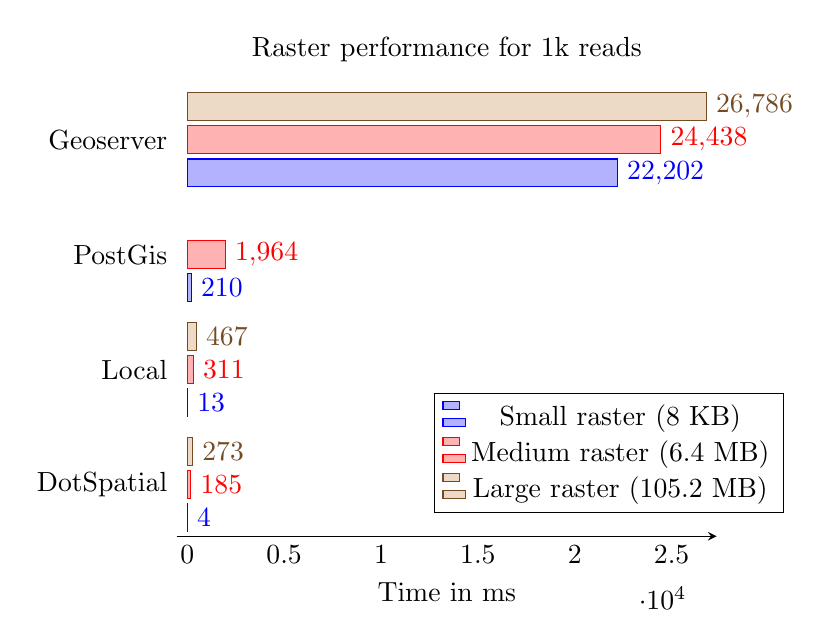
\begin{tikzpicture}
\begin{axis}[
title  = Raster performance for 1k reads,
xbar,
y axis line style = { opacity = 0 },
axis x line       = bottom,
tickwidth         = 0pt,
enlarge y limits  = 0.15,
enlarge x limits  = 0.02,
symbolic y coords = {DotSpatial, Local, PostGis, Geoserver},
nodes near coords,
legend style={at={(0.8,0.32)},anchor=north},
xlabel={Time in ms},
]
% Small Rasterfile
\addplot coordinates {
	(22202,Geoserver)
	(210,PostGis)
	(13,Local)
	(4,DotSpatial)
};
% Mid Rasterfile
\addplot coordinates {
	(24438,Geoserver)
	(1964,PostGis)
	(311,Local)
	(185,DotSpatial)
};
% Large Rasterfile
\addplot coordinates {
	(26786,Geoserver)
	(nan,PostGis) % 342197
	(273,DotSpatial)
	(467,Local)
};
\legend{Small raster (8 KB), Medium raster (6.4 MB), Large raster (105.2 MB)}
\end{axis}
\end{tikzpicture}
